\textbf{Human reference data.} The benchmark uses respondent-level VAS data for three short Japanese literary texts and four affect dimensions: interest, surprise, sadness, and anger. The three works are Kyusaku Yumeno's \textit{The Pocket Watch} (T1; \textit{Kaichu dokei}), Kyusaku Yumeno's \textit{The Money and the Pistol} (T2; \textit{Okane to pisutoru}), and Kotaro Takamura's \textit{The Tattered Ostrich} (T3; \textit{Boroboro na dacho}). The task was administered in Japanese to student readers as a VAS survey in which each respondent rated the three texts on the same four emotions after reading each work. Ninety-one human responses were collected, of which 86 were complete cases retained for the primary aggregate reference profile. The public repository stores only sanitized numeric derivatives. The present analysis reuses only anonymized secondary numeric derivatives of the student VAS data; raw survey exports and platform metadata are not redistributed.

\textbf{Texts and model panel.} The computational benchmark evaluates the same three works used in the human task and compares six contemporary LLMs from six major providers: Claude Sonnet 4.5, GPT-5.4, Grok 4.20, Qwen3.6 Plus, DeepSeek V3.2, and Gemini 2.5 Pro. Each model was queried in Japanese, English, and Chinese. The model panel was intentionally kept compact to match the engineering-pilot scope of the paper while preserving vendor diversity.

\textbf{Task definition.} The neutral-reader model run operationalized the same four affect dimensions on a 0--100 scale to approximate the human VAS task. One LLM experimental unit consisted of one model, one language, one text, one neutral-reader prompt, and one repetition. The model received the full literary text, the neutral-reader role, the four emotion definitions, and the scoring rule that 0 means the emotion is not felt at all, 50 means moderately felt, and 100 means extremely strongly felt. It returned one JSON object containing four integer scores and brief text-grounded reasons. A single neutral-reader prompt was used in all languages so that the benchmark would remain interpretable as a human-alignment pilot rather than collapse back into persona-conditioned evaluation. Japanese human alignment is the primary endpoint because the reference VAS data were collected in Japanese, with Japanese source texts and Japanese task instructions used in the primary human--LLM alignment condition. English and Chinese are therefore not treated as co-equal human-grounded evaluations but as cross-language robustness tests; in those runs, both the literary texts and the task instructions were language-matched using fixed author-prepared translations, so drift reflects the combined effect of translated text and prompt language rather than instruction language alone. Because the benchmark is intentionally compact, the analysis is interpreted descriptively for screening utility rather than formal significance testing. This design keeps persona-conditioned prompting outside the center of the present paper, because persona and temperature were confounded in our earlier LLM-only design \cite{shirahama2026mdpi}.

\begin{figure*}[t]
\centering
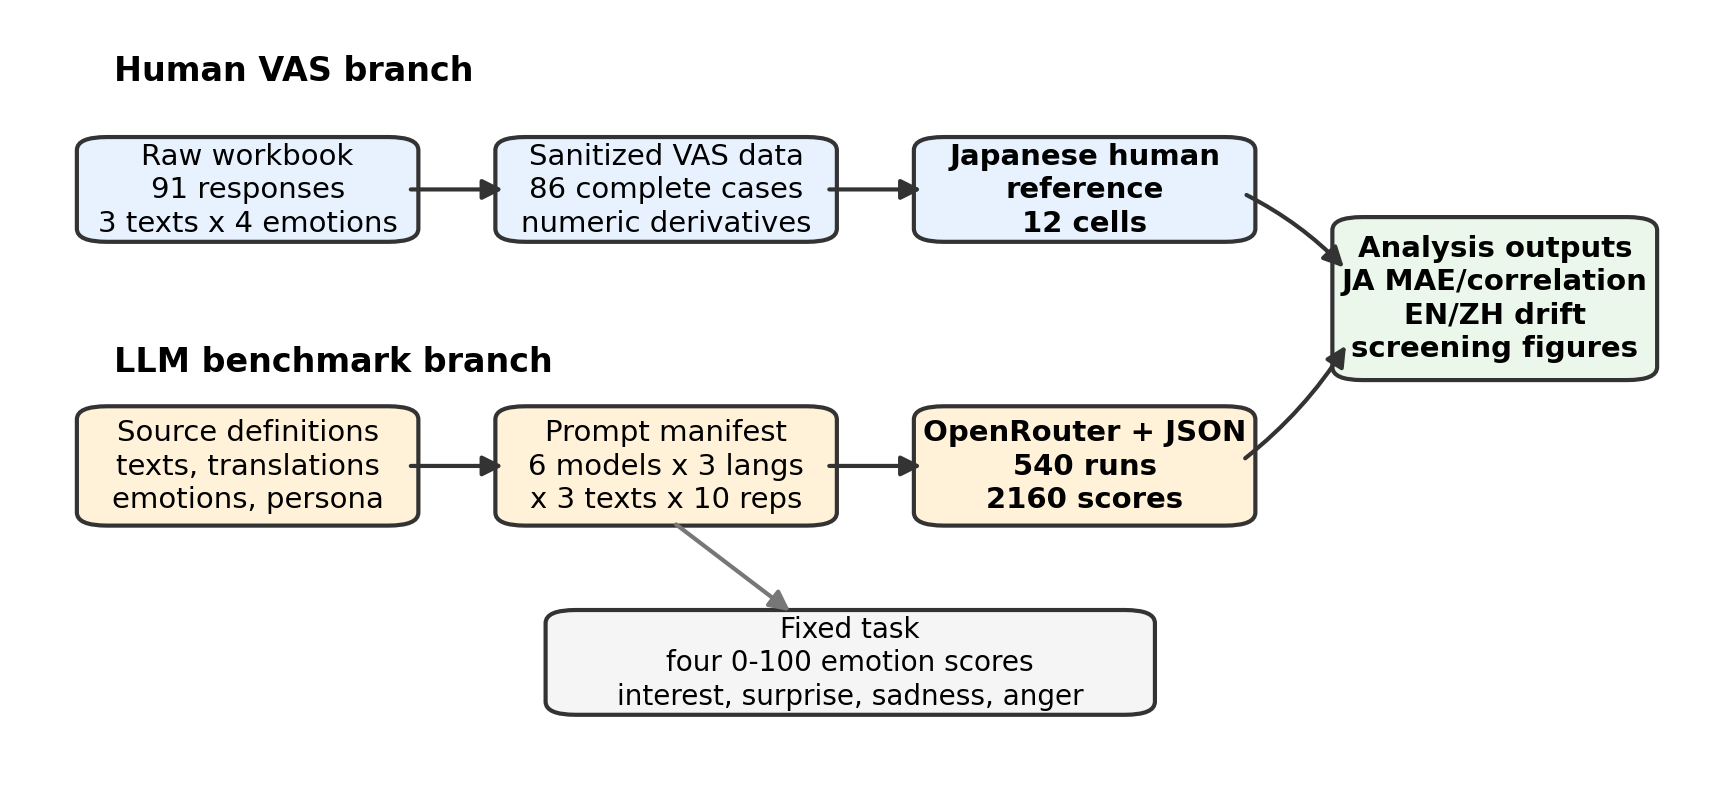
\includegraphics[width=0.96\textwidth]{fig/figure1_system_workflow.pdf}
\caption{System configuration and data flow for the benchmark. The human branch converts the private Japanese VAS workbook into sanitized story-by-emotion reference cells. The LLM branch combines the fixed source definitions, translated texts, prompt template, response schema, and model manifest to run the neutral-reader benchmark through OpenRouter. The analysis compares Japanese model profiles with the human reference and treats English and Chinese as cross-language robustness conditions.}
\label{fig:workflow}
\end{figure*}

\textbf{Aggregation.} Let $s \in \{1,2,3\}$ index texts and $d \in \{1,2,3,4\}$ index affect dimensions. The Japanese human reference profile is
\begin{equation}
H_{s,d}=\frac{1}{N_s}\sum_{i=1}^{N_s} y_{i,s,d},
\end{equation}
where $y_{i,s,d}$ is the VAS score from respondent $i$ and $N_s$ is the number of complete human responses for text $s$. For model $m$, language $\ell \in \{\mathrm{JA},\mathrm{EN},\mathrm{ZH}\}$, and repetition count $R=10$, the aggregated model profile is
\begin{equation}
M_{m,\ell,s,d}=\frac{1}{R}\sum_{r=1}^{R} x_{m,\ell,s,d,r}.
\end{equation}
This yields a 12-value story-by-emotion profile for each model-language condition.

\textbf{Metrics.} The primary endpoint is Japanese human alignment. For each model, Japanese scores were aggregated to a story-by-emotion profile and compared against the Japanese human reference using mean absolute error (MAE), Pearson correlation, and Spearman rank correlation:
\begin{equation}
\mathrm{MAE}_{m,\mathrm{JA}}=\frac{1}{12}\sum_{s,d}\left|M_{m,\mathrm{JA},s,d}-H_{s,d}\right|.
\end{equation}
English and Chinese were not treated as additional human-grounded endpoints. Instead, cross-language drift was defined as the mean absolute difference between each model's English or Chinese story-by-emotion score profile and the same model's Japanese profile:
\begin{equation}
D_{m,\ell}=\frac{1}{12}\sum_{s,d}\left|M_{m,\ell,s,d}-M_{m,\mathrm{JA},s,d}\right|,~~
\ell \in \{\mathrm{EN},\mathrm{ZH}\}.
\end{equation}
We also report the average drift
\begin{equation}
\bar{D}_m=\frac{D_{m,\mathrm{EN}}+D_{m,\mathrm{ZH}}}{2}.
\end{equation}
Lower MAE and lower drift are better. Because the benchmark is intentionally compact, the paper emphasizes descriptive comparison and screening utility rather than formal significance testing.

\textbf{Protocol and reproducibility.} The protocol comprised 91 human responses, with 86 complete cases retained for the primary aggregate reference profile, across 3 texts and 4 affect dimensions. The model side covered 6 models $\times$ 3 languages $\times$ 3 texts $\times$ 10 repetitions under one neutral-reader prompt, yielding 540 neutral-reader model runs and 2160 numeric scores. Figure~\ref{fig:workflow} summarizes the two data branches and the downstream analysis. For reproducibility, the public repository stores only sanitized numeric derivatives of the student VAS data, while raw survey exports and platform metadata are not redistributed.

\begin{table}[t]
\caption{Primary benchmark design summary.}
\label{tab:design}
\centering
\begin{tabular}{lr}
\toprule
Item & Value \\
\midrule
Human responses & 91 \\
Complete cases & 86 \\
Texts & 3 \\
Affect dimensions & 4 \\
Models & 6 \\
Languages & 3 (JA/EN/ZH) \\
Prompt condition & 1 (neutral reader) \\
Repetitions per condition & 10 \\
Total neutral-reader model runs & 540 \\
Total numeric scores & 2160 \\
\bottomrule
\end{tabular}

\end{table}
